\mychapter{5}{Análisis y Desarrollo Experimental}

En este capítulo voy a hacer una recapitulación de la estructura y desarrollo de los experimentos que se han llevado a cabo para la realización de este TFG, además de una breve exlicación de las distintas herramientas que se han utilizado para ello.\\

\section{Máquinas en las que se han realizado los experimentos}

Las dos máquinas principales en las que se han realizado los experimentos han sido las siguientes:
\begin{itemize}
	\item \textbf{MacBook Air 2016}: \textit{Procesador}, 1,6 GHz Intel Core i5. \textit{Memoria},8 GB 1600 MHz DDR3. Principalmente utilizado para el procesamiento de las imágenes NIFTI.
	\item \textbf{Servidor}: \textit{Procesadores}, 2 Intel(R) Xeon(R) CPU   E5645  @ 2.40GHz. \textit{GPU}, 2 Tesla C2050 / C2075. Utilizada para la realización de los experimentos.
\end{itemize}
\section{Herramientas utilizadas}

En primer lugar, quiero citar cuáles han sido las herramientas utilizadas para la realización de este trabajo.\\
\subsection{Librerías para trabajar con técnicas de Deep Learning }

Actualmente debido a los grandes avances que se han conseguido en ciertos campos con el uso de técnicas de Deep Learning. el número de librerías dedicadas a facilitar la realización de experimentos con este tipo de técnicas ha crecido a una gran velocidad, dejándonos muchas opciones donde elegir.\\

Existe un abanico muy amplio de librerías donde elegir, entre ellas hay librerías que llevan más tiempo como por ejemplo \textbf{Caffe}\cite{Caffe} o \textbf{Theano}\cite{Theano} y otras cuyo tiempo de vida es menor. En este último grupo encontramos una librería que en los últimos años ha tenido mucha repercusión, la cuál es \textbf{Tensorflow}\cite{Tensorflow}. Su gran crecimiento puede deberse a varios factores, entre ellos su rapidez (dentro de lo posible) en tiempos de computación,y que viene de la mano de Google.\\

La mayoría de estas librerías requiere mucho conocimiento técnico de lo que se está haciendo y controlar a mano muchos parámetros que pueden suponernos un retraso a la hora de la realización de los experimentos, debido a necesitar tiempo para arreglar fallos dentro del código.\\

Es por estos motivos por los que François Chollet, un trabajador de Google, creó la \textit{high-level API} \textbf{Keras}\cite{keras}. Keras, es una librería que nos sirve como capa para la utilización tanto de Tensorflow como Theano. Nos permite, por ejemplo, métodos automáticos para el entrenamiento utilizando un número fijado de \textit{batch}, mientras que en Tensorflow o Theano tendríamos que programar esto a mano. Este tipo de ayudas permite que el tiempo que se requiere desde el momento en el que comienzas a programar un experimento hasta el fin de su ejecución sea el más rápido posible y lo más ausente de fallos.\\

Es por estas, y más razones, que se ha decido utilizar \textbf{Keras} como librería para trabajar con técnicas de Deep Learning.\\
\begin{figure}[H]
	\label{figure1}
	\centering
	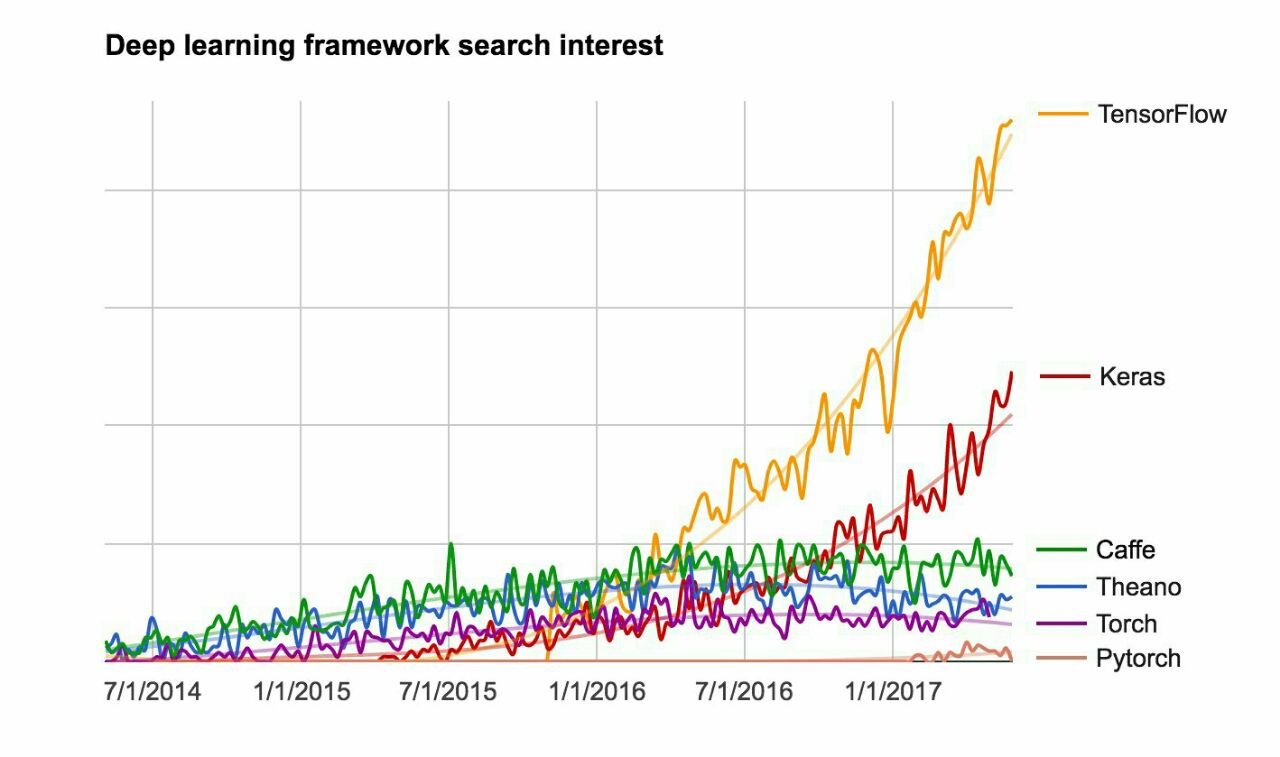
\includegraphics[width=350px]{imagenes/dlsearch.jpg}
	\caption{Interés de búsqueda de Frameworks de Deep Learning. Fuente: François Chollet}
\end{figure}

\begin{figure}[H]
	\label{figure1}
	\centering
	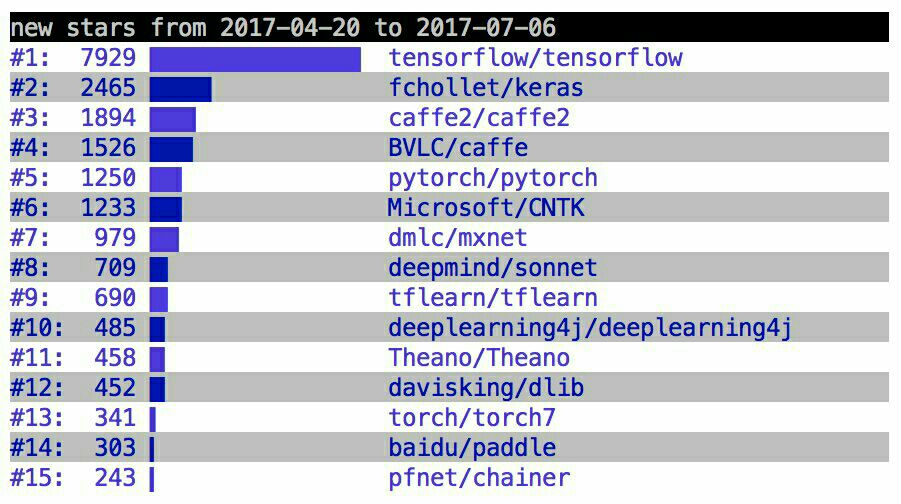
\includegraphics[width=\textwidth]{imagenes/dlstars.jpg}
	\caption{Stars a repositorios de Github. Fuente: François Chollet}
\end{figure}

\subsection{Librería para trabajar con las imágenes en formato NIFTI}
\label{nibabel}
Para poder trabajar con redes convolucionales en 2 dimensiones, debido a que la capacidad de computación requerida para trabajar con las imágenes en 3D no era posible, se requería una librería con la que poder obtener las capas del cerebro que nosotros quisiésemos y luego guardarlas en un formato con el que Keras pudiese tratar.\\
Para ello, se utilizó la librería para Python \textbf{Nibabel}\cite{Nibabel}. Esta librería nos permite obtener toda la información de un archivo NIFTI y poder coger el \textbf{slice} que queramos.\\
\section{Procesamiento de las imágenes NIFTI}
\label{procesamiento-imagenes}
En nuestro caso, se requería previamente obtener imágenes 2D a partir de laos archivos NIFTI. Esto era necesario a la hora de poder tratar estas imágenes con Keras, para la realización de los experimentos.Para ello, se creó un script llamado \textit{create\_slices.py}.\\

Con este script lo que se consigue es la lectura de todos los archivos NIFTI, obteniéndose las capas desde la 10 a la 100 de 5 en 5, y guardándose ordenadamente en una nueva carpeta correspondiente a cada capa, obteniendo 19 carpetas distintas.\\

Se guardan en esta estructura para luego poder leerlos ordenadamente y obtener resultados sobre cada slice del cerebro. Con esto se nos permitirá determinar cuál es la capa del
cerebro que mejor resultados nos da.\\
\section{Arquitectura de la CNN  \ref{CNN}}

Esta es una decisión muy importante a la hora de la realización del TFG. Para ello se revisó la bibliografía más reciente, para partir de una base sólida a la hora de la elección del modelo. En la revisión bibliográfica podemos encontrar estudios como \cite{residualVGG} y \cite{SarrafT16}.\\

Por parecernos más concluyentes los resultados de \cite{residualVGG} debido a la metodología de separación de pacientes que ellos utilizaban, se decidió utilizar la primera arquitectura que ellos introducen, basada en la arquitectura \textbf{VGG} \cite{SimonyanZ14a}.\\

La arquitectura podemos observarla en la Figura \ref{arquitectura}. En nuestro caso, se ha modificado para que sea una red que acepte entradas 2D en lugar de 3D.\\

En el artículo \cite{residualVGG} también se prueba otro tipo de arquitectura, un tipo de arquitectura residual. Pero en los resultados no se encuentra una mejora sustancial como para aplicar una arquitectura más compleja, y que requiera más tiempo de computación.\\
\section{Experimentos}

En esta sección, se irán explicando los distintos experimentos que se han llevado a cabo para el estudio de métodos para la clasificación de las imágenes en 2D y cuál sería la mejor estrategia para el análisis de las mismas, eligiendo la capa del cerebro más significativa para la clasificación.\\
\subsection{Parámetros comunes a todos los experimentos}

Hay unos parámetros comunes que se han utilizado para todos los experimentos, los cuáles se relatan a continuación.\\

Con respecto a la arquitectura, se ha utilizado como función de \textit{loss} la función \textbf{categorical cross-entropy} y un \textit{learnig rate} de \textbf{$27\times 10^{-6}$}.\\

Además, en cuanto al entrenamiento se refiere, se ha utilizado un número de \textit{epochs} igual a 70 y un \textit{batch size} de 5.\\
\subsection{Experimentos previos a los tres experimentos finales}

Al inicio comenzamos trabajando con una sola capa de todas las imágenes y se decidió utilizar la capa media del cerebro. En nuestro caso, al ser las imágenes de \textbf{110x110}. Como tenemos un conjunto de datos reducido, ya que solo disponemos de 389 imágenes y este número en términos de usar técnicas de Deep Learning es tener un conjunto de datos muy pequeño, decidimos usar técnicas de validación para poder determinar si los resultados obtenidos eran significativos o no. Para intentar emular los resultados del artículo \cite{residualVGG} previamente citado, se redujo el conjunto de datos al utilizar solo una imagen por paciente, ya que hay pacientes de los cuáles disponemos más de una imagen de distinto período temporal, dejando el conjunto de datos a una cantidad de 131 imágenes. Para ello se implementó un \textit{5-Fold Cross Validation}, ya que es lo que se utilizó en \cite{residualVGG} y además nos da una robustez en los resultados.\\

Viendo el desempeño que había tenido con el conjunto reducido se decidió comprobar si aumentando el número de imágenes se obtendrían mejores resultados. Esto quiere decir, utilizando todas las imágenes de los pacientes, pero siempre comprobando que no ocurra el caso en que dos imágenes distintas de un paciente se encuentre en \textit{train} y en \textit{test} al mismo tiempo. Para ello se hizo una separación manual de las imágenes en 5 \textit{folds} para la realización al igual que anteriormente de un \textit{5-fold Cross Validation}, siempre respetando la restricción anteriormente explicada y se obtuvo una mejora en los resultados.\\

En este momento, se pensó que quizá con otras capas se podrían llegar a mejores resultados, porque la red en esas imágenes aprendiese unos mejores filtros. Es por esto que se decidió utilizar otras capas para comprobar si existían diferencias.\\

Viendo que los resultados variaban según la capa que utilizases, decidimos responder a la pregunta, ¿cuál será la capa que mejor rendimiento nos dé a la hora de clasificar entre pacientes normales y pacientes con Alzheimer?. Con esto habríamos determinado que se puede hacer una clasificación de estos pacientes con CNN y que, además, hay ciertas capas dentro de una imagen tridimensional que nos ayudan a clasificar mejor a un paciente.\\

Como último dato, decir que también se aplicó otra alternativa para ver si había una correlación entre las imágenes de los pacientes o eran muy diferentes unas y otras. Se utilizó un \textit{5-Fold Cross Validation} sin asegurarse de que no se repetían distintas imágenes de los pacientes en distintos conjuntos, obteniendo resultados formidables. Esto no sirve sino para reforzar la idea de que no podemos usar imágenes del mismo paciente en distintos conjuntos, ya que puede llevar a la filtración de características que hagan más fácil la tarea de la red a la hora de clasificar.\\

\subsection{Experimento 1: Leaving-one-out Cross Validation con todas las imágenes}
\label{exp1}
El primer experimento a realizar se usó para confirmar la teoría de que hay filtración de información entre imágenes, junto con los resultados de experimento 2. En este caso, no se realizó ninguna separación de las imágenes de los pacientes, sino que se trataron como si todas fuesen imágenes distintas.\\

Es necesario añadir que el tiempo de ejecución de este experimento fue de alrededor de unas 28 horas, ya que la técnica de validación de \textit{LOO Cross-Validation} es muy demandante en cuanto a tiempo se refiere. A continuación, con el segundo experimento se iba a comprobar si de verdad existía una filtración de información entre imágenes del mismo paciente.\\
\newpage
\begin{figure}[H]
	\centering
	\caption{Arquitectura utilizada basada en la arquitectura VGG \cite{SimonyanZ14a} del artículo \cite{residualVGG}}
	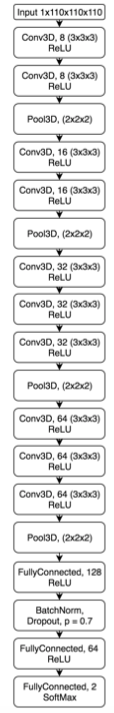
\includegraphics[height=\textheight]{imagenes/model.png}
	\label{arquitectura}
\end{figure}

\subsection{Experimento 2: Leaving-one-out Cross Validation por paciente}
\label{exp2}
Con este experimento, lo que se intentaba era comprobar si de verdad había una filtración de información entre las imágenes de los pacientes usando un método de validación más robusto como es el \textit{LOO Cross-Validation}.\\

Para ello lo que se realizó fue una implementación especial del algoritmo de \textit{LOO Cross-Validation} en el que en lugar de sacar en cada iteración un elemento al conjunto de \textit{test}, se meten en \textit{test} todas las imágenes que pertenece al mismo paciente paciente, gracias a un vector que contiene el número de identificación del paciente. Además, se lleva un registro de los pacientes que ya se han introducido en \textit{test} para que cuando se continúe con el entrenamiento y nos encontramos con otra imagen del mismo paciente no se vuelva a realizar lo mismo que se ha realizado previamente.\\
\subsection{Experimento 3:  5-Fold Cross Validation para ver cuál es la mejor capa}

Una vez realizados los experimentos previos decidimos responder a la pregunta, ¿cuál será la capa del cerebro con la que se obtienen mejores resultados?. Por lo tanto, se realizó un \textit{5-Fold Cross Validation} para comprobar cuál es la capa que mayor rendimiento obtiene en cuanto a \textit{accuracy} en el conjunto de \textit{test}.\\

La separación de los pacientes se realizó manualmente, para asegurarnos de que no hubiese imágenes del mismo paciente en distintos conjuntos. Esto nos dejó con 4 conjuntos compuestos pro 77 imágenes y el último compuesto por 76 imágenes.